\documentclass[tikz,border=10pt]{standalone}
\usepackage{tikz}
\usepackage{amsmath} % Provides \text{} in math mode
\usetikzlibrary{shapes,arrows.meta,positioning,calc,fit} % Added fit library

\begin{document}

% ------------------------------------------------------------------
% 1. LOCK-IN AMPLIFIER SCHEMATIC
% ------------------------------------------------------------------
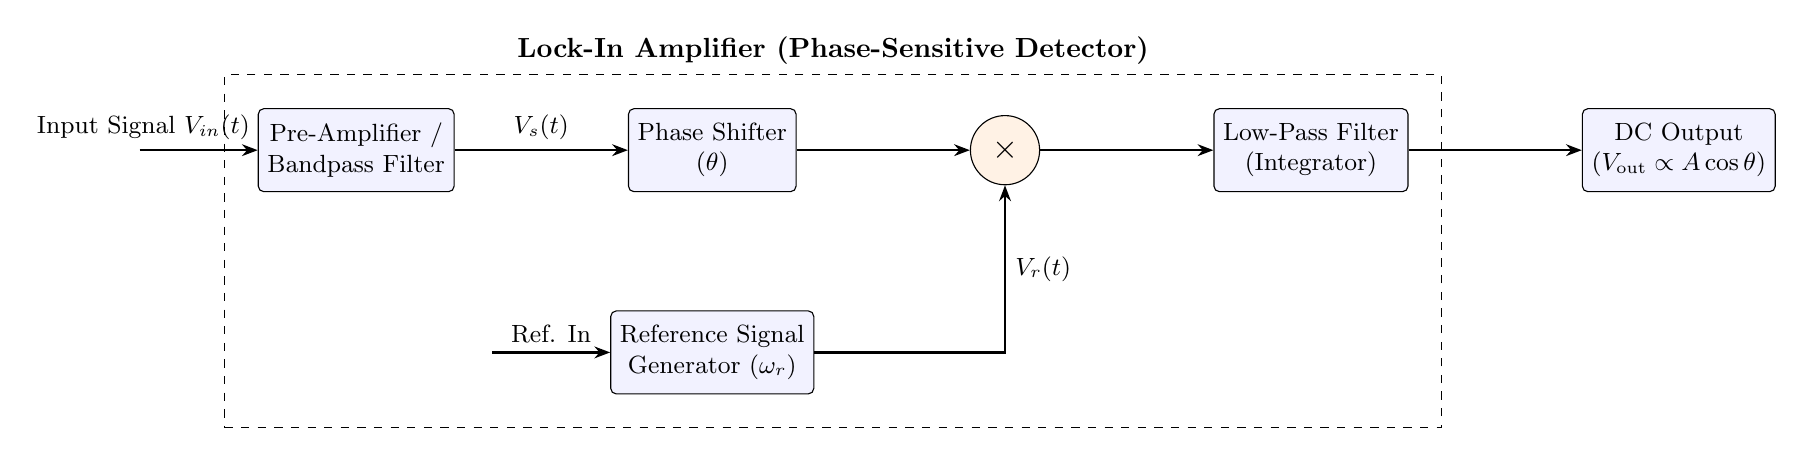
\begin{tikzpicture}[
    block/.style = {draw, rectangle, minimum height=3em, minimum width=4.5em, align=center, fill=blue!5, rounded corners=2pt, font=\small},
    circleblock/.style = {draw, circle, minimum size=2.5em, fill=orange!10, font=\large},
    signal/.style = {-{Stealth[length=2mm]}, thick},
    node distance = 1.8cm and 2.2cm
]

\node [block] (input_amp) {Pre-Amplifier /\\ Bandpass Filter};
\node [block, right=of input_amp] (phase_shifter) {Phase Shifter\\ ($\theta$)};
\node [circleblock, right=of phase_shifter] (mixer) {$\times$};
\node [block, right=of mixer] (lpf) {Low-Pass Filter\\ (Integrator)};
\node [block, right=of lpf] (output) {DC Output\\ ($V_{\text{out}} \propto A \cos\theta$)};

% Reference Channel
\node [block, below=1.5cm of phase_shifter] (ref_gen) {Reference Signal\\ Generator ($\omega_r$)};

% Connections
\draw [signal] ([xshift=-1.5cm]input_amp.west) -- node[above, xshift=-20, font=\small] {Input Signal $V_{in}(t)$} (input_amp);
\draw [signal] (input_amp) -- node[above, font=\small] {$V_s(t)$} (phase_shifter);
\draw [signal] (phase_shifter) -- (mixer);
\draw [signal] (mixer) -- (lpf);
\draw [signal] (lpf) -- (output);

\draw [signal] ([xshift=-1.5cm]ref_gen.west) -- node[above, font=\small] {Ref. In} (ref_gen);
\draw [signal] (ref_gen) -| node[near end, right, font=\small] {$V_r(t)$} (mixer);

% Surrounding Box
\node[draw, dashed, inner sep=12pt, label=above:{\bf Lock-In Amplifier (Phase-Sensitive Detector)}, fit=(input_amp) (phase_shifter) (mixer) (lpf) (ref_gen)] {};

\end{tikzpicture}

\vspace{1cm}

% ------------------------------------------------------------------
% 2. BOXCAR AVERAGER SCHEMATIC
% ------------------------------------------------------------------
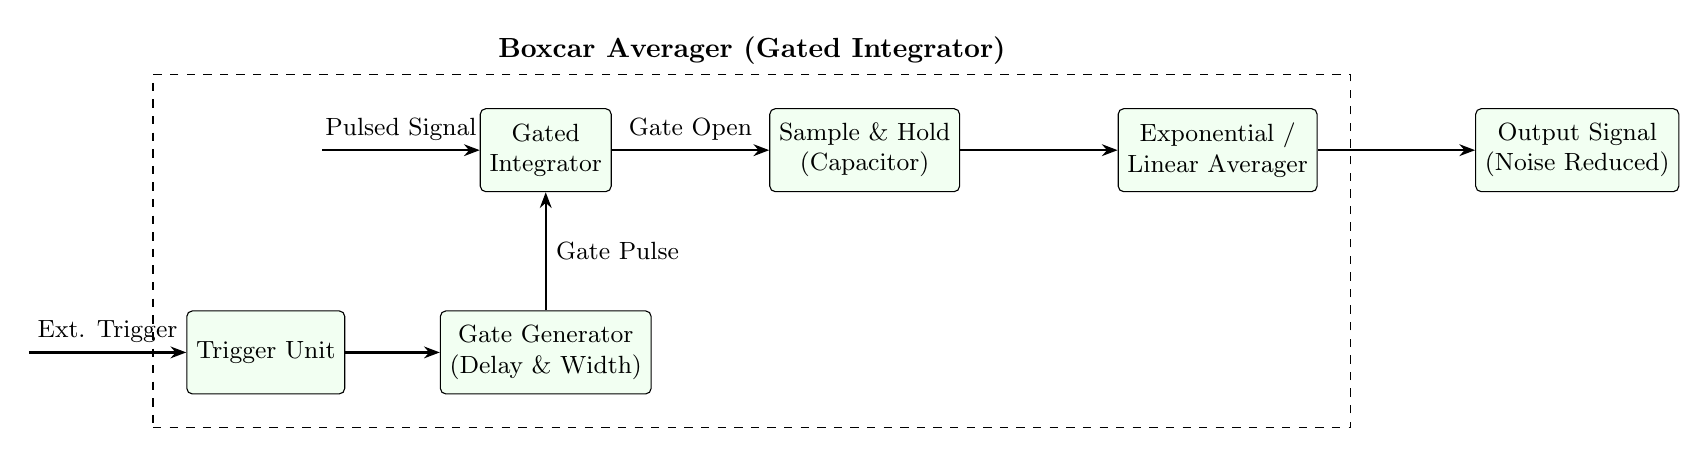
\begin{tikzpicture}[
    block/.style = {draw, rectangle, minimum height=3em, minimum width=4.5em, align=center, fill=green!5, rounded corners=2pt, font=\small},
    switch/.style = {draw, circle, inner sep=1.5pt, fill=black},
    signal/.style = {-{Stealth[length=2mm]}, thick},
    node distance = 1.8cm and 2cm
]

\node [block] (input_amp) {Gated\\ Integrator};
\node [block, right=of input_amp] (hold) {Sample \& Hold\\ (Capacitor)};
\node [block, right=of hold] (avg) {Exponential /\\ Linear Averager};
\node [block, right=of avg] (output) {Output Signal\\ (Noise Reduced)};

% Trigger and Gate Generator
\node [block, below=1.5cm of input_amp] (gate_gen) {Gate Generator\\ (Delay \& Width)};
\node [block, left=1.2cm of gate_gen] (trigger) {Trigger Unit};

% Connections
\draw [signal] ([xshift=-2cm]input_amp.west) -- node[above, font=\small] {Pulsed Signal} (input_amp);
\draw [signal] (input_amp) -- node[above, font=\small] {Gate Open} (hold);
\draw [signal] (hold) -- (avg);
\draw [signal] (avg) -- (output);

\draw [signal] ([xshift=-2cm]trigger.west) -- node[above, font=\small] {Ext. Trigger} (trigger);
\draw [signal] (trigger) -- (gate_gen);
\draw [signal] (gate_gen) -- node[right, font=\small] {Gate Pulse} (input_amp);

% Surrounding Box
\node[draw, dashed, inner sep=12pt, label=above:{\bf Boxcar Averager (Gated Integrator)}, fit=(input_amp) (hold) (avg) (gate_gen) (trigger)] {};

\end{tikzpicture}
\end{document}
